Para alcanzar esa meta a�n queda un largo camino que recorrer. Los trabajos hasta la fecha han supuesto un enorme avance y adem�s se ha logrado en un periodo de tiempo relativamente corto. Como ya se ha comentado, tanto las tecnolog�as de secuenciaci�n como los sistemas de clasificaci�n no son perfectos todav�a e introducen errores en los resultados. Adem�s, se ha demostrado que los intentos de explicar las relaciones entre microorganismos mediante correlaciones no muestran las verdaderas interacciones \cite{Fisher2014}. En ese mismo art�culo, los autores proponen una aproximaci�n capaz de superar todos esos obst�culos a la que han llamado LIMITS (detallada en Materiales y m�todos). Para comprobar su potencial y comparar los resultados expuestos en apartados anteriores, se aplic� LIMITS a los datos del estudio. En la figura \ref{LIMITS_salivaA} se puede observar la matriz de interacciones propuesta para saliva A, en la figura \ref{LIMITS_intestinoA} para intestino A y en la figura \ref{LIMITS_intestinoB} para intestino B.

\begin{figure}[!h]
    \centering
    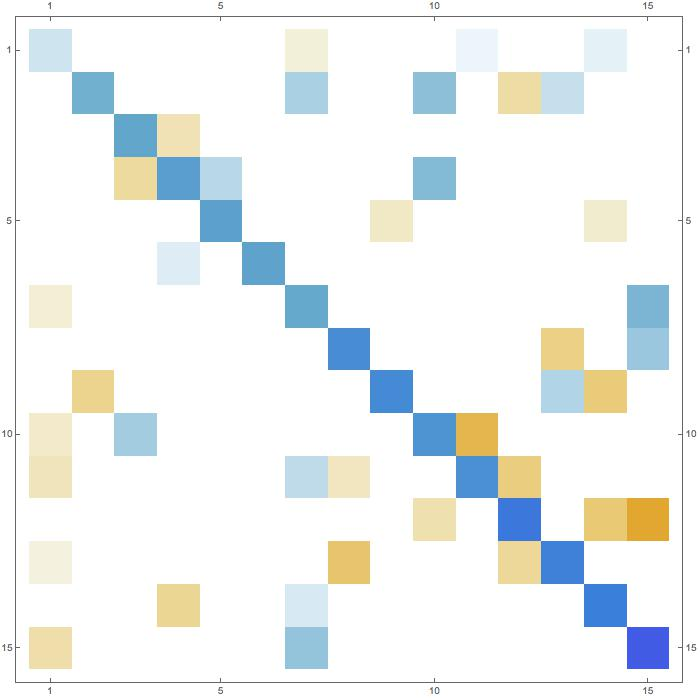
\includegraphics[width=4.5in]{./Figuras/SalivaA_15otus_alltimes.jpg}
    \caption{LIMITS saliva A}
    \label{LIMITS_salivaA}
\end{figure}

\begin{figure}[!h]
    \centering
    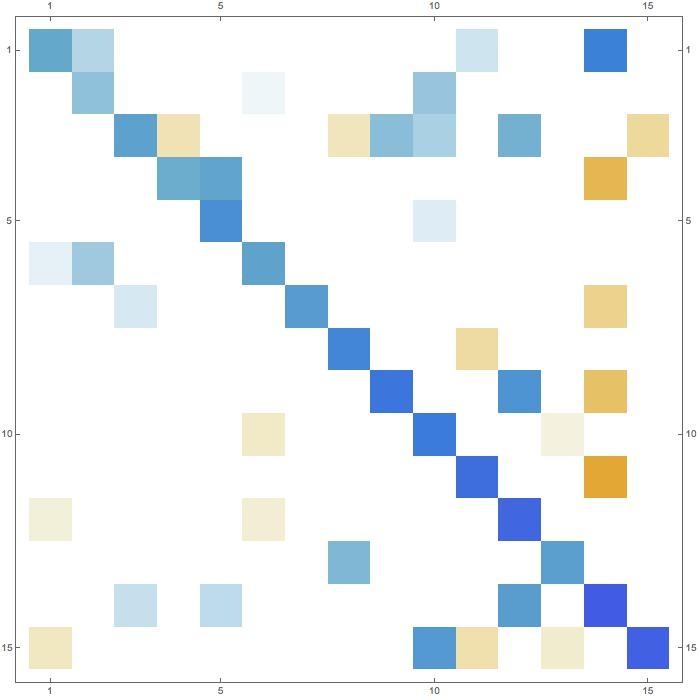
\includegraphics[width=4.5in]{./Figuras/StoolA_15otus_alltimes.jpg}
    \caption{LIMITS intestino A}
    \label{LIMITS_intestinoA}
\end{figure}

\begin{figure}[!h]
    \centering
    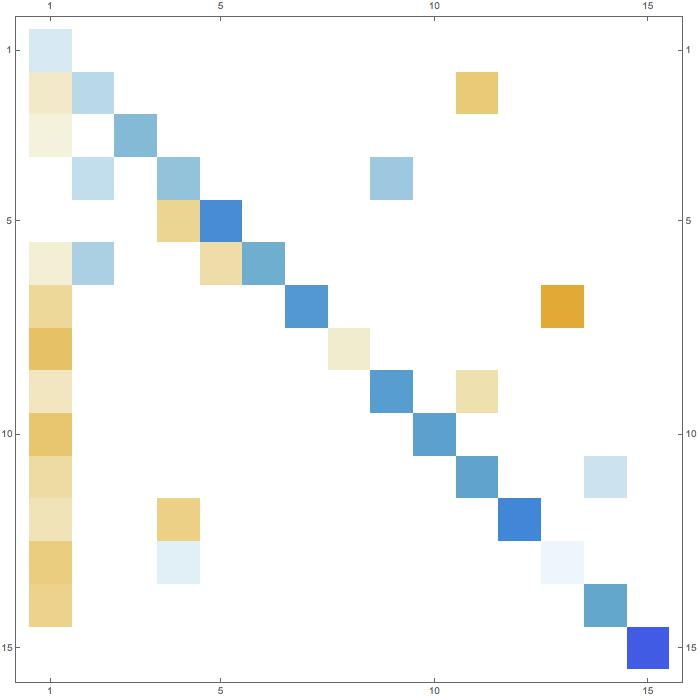
\includegraphics[width=4.5in]{./Figuras/StoolB_15otus_alltimes.jpg}
    \caption{LIMITS intestino B}
    \label{LIMITS_intestinoB}
\end{figure}